\documentclass{article}


\usepackage{lmodern}
\usepackage[T1]{fontenc}
\usepackage[spanish,activeacute]{babel}
\usepackage{mathtools}
\usepackage{subfig}
\usepackage{graphicx}
\usepackage{listings}
\usepackage{float}

\begin{document}

\begin{figure}[htbp]

\includegraphics{logo_latex} 
\end{figure}

\textbf{\Huge{Informe de Tarea \#3}}\\[0.2cm]
\textbf{\Huge{Redes de Computadores}}
\\ \ \\ \

\begin{flushleft}
\large{\textbf{Profesor:}} 
\large{Oscar Encina Calqu'in} 
\\ \


\large{\textbf{Integrantes:}} \par
\large{Felipe Araya Barrera  201173501-3  felipe.araya@alumnos.usm.cl}\\ \

\large{Felipe Berrios Toloza  201173501-3 felipe.berrios@alumnos.usm.cl}\\

\end{flushleft}

\newpage

\section{Introducci'on}
En el siguiente informe se trabajar'a sobre la capa de red, para ello se utilizar'a el programa Open Visual Traceroute el cual nos permitir'a rastrear la ruta de un paquete de datos desde la ubicaci'on del env'io hasta el servidor de destino.

\section{Recorrido de los paquetes}
En primer punto se usar'a OVT para observar que sucede con las direcciones escogidas. El servidor de inicio ser'a el de mi hogar:

\subsection{http://moodle.inf.usm.cl/}
Primero se revisar'a el recorrido del link del moodle de nuestra universidad:
\\
\begin{figure}[H]
  \centering
    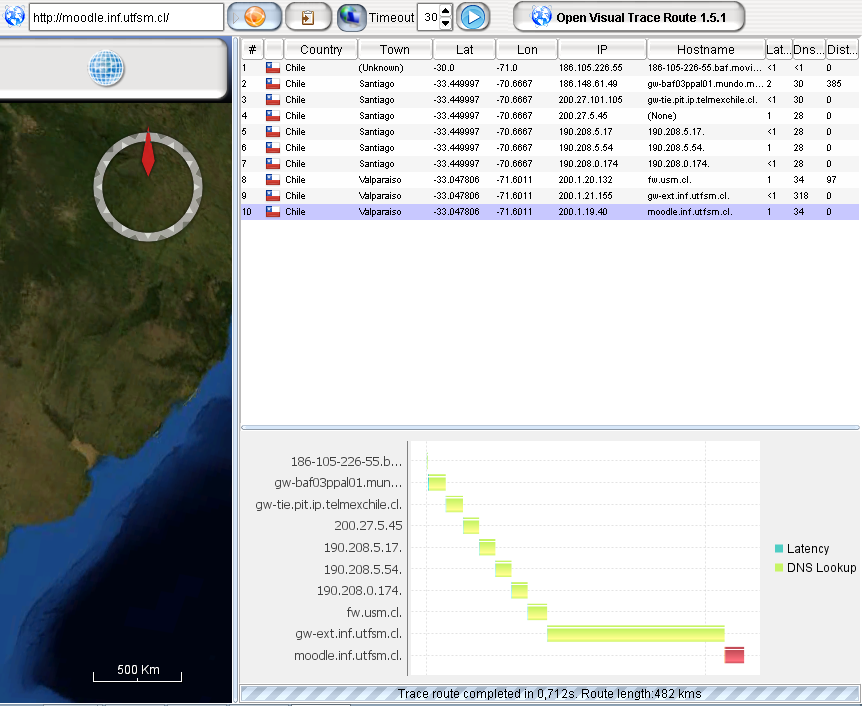
\includegraphics[width=1.0\textwidth]{ruta1_moodle}
  \caption{Recorrido link Moodle}
  \label{moodle}
\end{figure}

El tiempo del recorrido de la ruta dura 0,712 segundos con un recorrido total en orden desde Santiago a Valpara'iso de 482 kil'ometros.

\subsection{http://google.cl/}
Luego se proceder'a a revisar el recorrido hecho por el buscador Google:
\\
\begin{figure}[H]
  \centering
    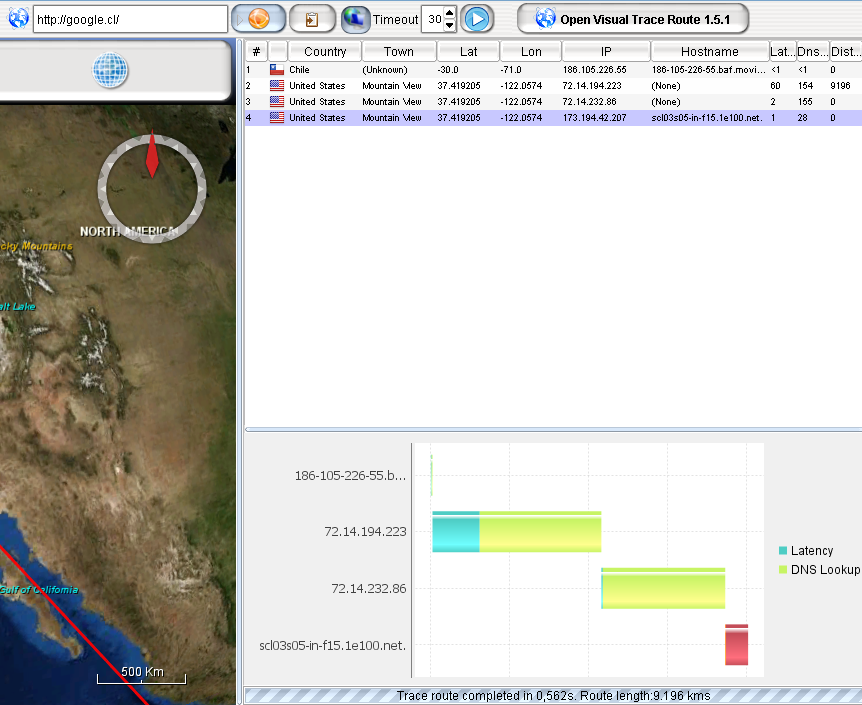
\includegraphics[width=1.0\textwidth]{ruta1_google}
  \caption{Recorrido link Google}
  \label{google}
\end{figure}

El tiempo del recorrido de la ruta dura 0,562 segundos con un recorrido total en orden desde Santiago a Mountain View, Estados Unidos de 9.196 kil'ometros.
\newpage
\subsection{http://cime.cl/}
La tercera p'agina a revisar ser'a la del Cime:
\\
\begin{figure}[H]
  \centering
    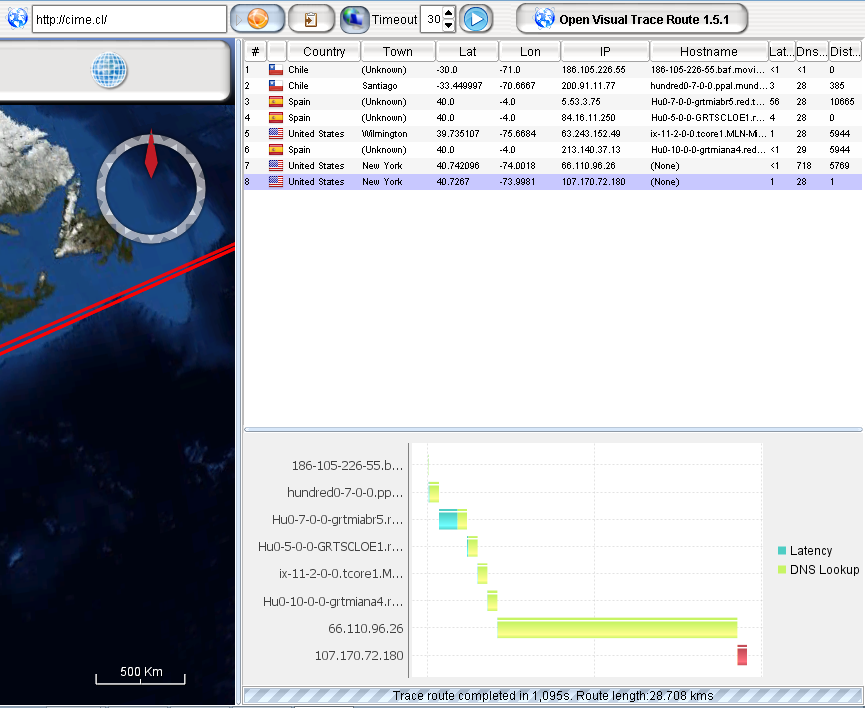
\includegraphics[width=1.0\textwidth]{ruta1_cime}
  \caption{Recorrido link Cime}
  \label{cime}
\end{figure}

El tiempo del recorrido de la ruta dura 1,095 segundos con un recorrido total en orden desde Santiago a Espa\~na, Estados Unidos, nuevamente a Espa\~na, regresando finalmente a Estados Unidos de 28.708 kil'ometros.
\newpage
\subsection{http://wikipedia.com/}
El recorrido de Wikipedia es el siguiente:
\\
\begin{figure}[H]
  \centering
    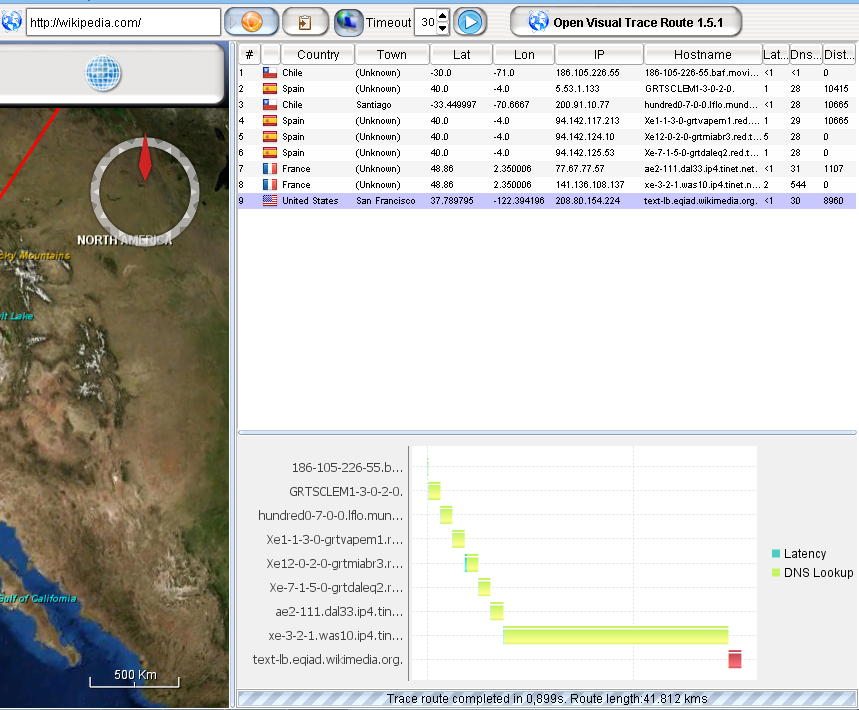
\includegraphics[width=1.0\textwidth]{ruta1_wikipedia}
  \caption{Recorrido link Wikipedia}
  \label{wikipedia}
\end{figure}

El tiempo del recorrido de la ruta dura 0,899 segundos con un recorrido total en orden desde Santiago a Espa\~na, regreso a Chile, nuevamente a Espa\~na, luego pasando por Francia y finalmente a San Francisco, Estados Unidos de 41.812 kil'ometros.
\newpage
\subsection{http://www.chile.embassy.gov.au/}
El recorrido de la p'agina de la embajada de Chile en Australia es el siguiente:
\\
\begin{figure}[H]
  \centering
    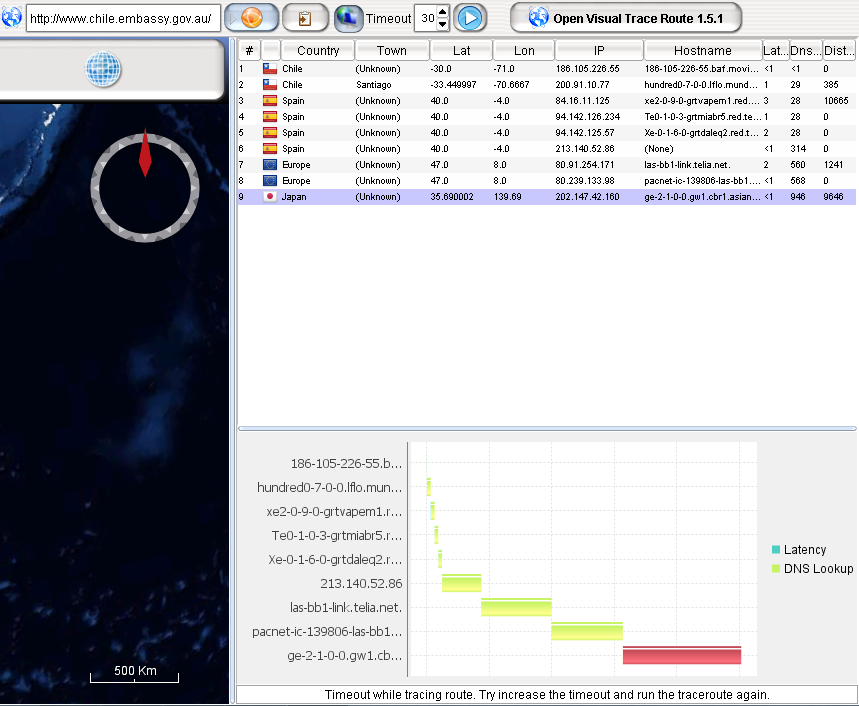
\includegraphics[width=1.0\textwidth]{ruta1_embchile}
  \caption{Recorrido link Embajada chilena en Australia}
  \label{embchile}
\end{figure}

Este recorrido tiene la peculiaridad de que despu'es de 30 segundos el recorrido llega a timeout, donde no llega al servidor destino, pese a que el paquete de datos viaja por Santiago, Espa\~na, una localidad de Europa y luego Jap'on.\\ \

En primera instancia, se aprecia que las rutas se realizan generalmente en tiempos muy cortos, adem'as llama la atenci'on que el tiempo del recorrido de la p'agina de Google es menor a la del moodle de nuestra universidad, considerando la gran distancia que hay entre pa'ises. Todo eso se ver'a con m'as profundidad en el siguiente punto.

\section{Los paquetes y las rutas}
En cada p'agina puesta a prueba por OVT se aprecia que los paquetes respectivos siguen diversas rutas, las cuales no son formadas al azar.\\ \
El Internet se compone de sistemas autónomos interconectados (AS en ingl'es). Un AS consiste t'ipicamente en muchas redes en el cual cada uno de ellos se administra de forma independiente.\\ \

La elecci'on del ruteo de los AS depende de protocolos de los cuales son 3 los m'as conocidos, RIP (Routing Information Protocol), OSPF (Open Shortest Path First) y IGRP (Interior Gateway Routing Protocol). Para el env'io de los paquetes de las p'aginas de esta tarea, se ahondar'a en OSPF.\\ \

OSPF fue concebido como el sucesor de RIP y, como tal, tiene una serie de caracter'isticas avanzadas. en su coraz'on, sin embargo, OSPF es un protocolo de estado de enlace que utiliza la inundaci'on de informaci'on de estado de enlace y al menos un algoritmo de Dijkstra de ruta de coste. Con OSPF, un router construye un mapa topol'ogico completo (es decir, un grafo dirigido) de todo el AS. El router entonces ejecuta localmente el algoritmo de Dijkstra para determinar el 'arbol de la ruta m'as corta a todas las redes con s'i mismo como el nodo ra'iz. La tabla de enrutamiento del router se obtiene de este 'arbol de la ruta m'as corta. Costos individuales de v'inculo se configuran por la red del administrador.\\ \

Con OSPF, un router env'ia peri'odicamente informaci'on de enrutamiento a todos los dem'as routers en el sistema aut'onomo, no s'olo a sus routers vecinos como el caso del protocolo RIP. De esta manera, cada uno de los paquetes es analizado, y a trav'es de Dijkstra (uno de los algoritmos vector distancia usados) se elige la menor distancia posible a recorrer.\\ \

Mediante el uso del programa OVT, es posible ver en cada link que pueden haber modificaciones en sus rutas cada vez que se revisa, esto es por la manera din'amica en la que se relacionan todos los routers y las conexiones. A'un as'i, la p'agina de la embajada de Chile en Australia es la 'unica con tener un timeout, ya que el env'io de los paquetes se anula con el firewall. Todas las dem'as p'aginas cumplen con sus tiempos respectivos y a pesar que algunas recorren mayores distancias donde se dirigen a diferentes continentes, su tiempo de viaje es menor al segundo, eso muestra que la efectividad del algoritmo es buena.\\ \
\section{Enlaces internacionales}
Los enlaces internacionales son la gran herramienta de la conectividad en el mundo. A trav'es de esto podemos conectarnos con el planeta, aqu'i se le muestra el mapa de cables submarinos:

\begin{figure}[H]
  \centering
    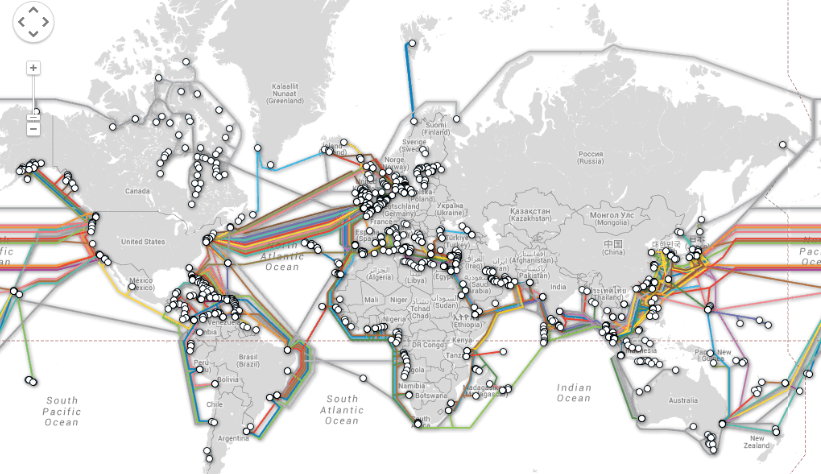
\includegraphics[width=1.0\textwidth]{mapamundo_enlaces}
  \caption{Mapa con las conexiones de cables submarinos en el mundo}
  \label{mapa}
\end{figure}

De estos enlaces, hay varios que se conectan con nuestro pa'is, los cuales son los siguientes:

\subsubsection{SAm-1}
SAm-1 (Sur Am'erica-1) es un cable submarino de fibra 'optica. Comenz'o sus operaciones en el a\~no 2000, conectando a Estados Unidos, Puerto Rico, Brasil, Argentina, Chile, Per'u y Guatemala. En el 2007, SAm-1 fue extendido a Ecuador y Colombia. Despu'es de su inmediata aprobaci'on en el 2000, consist'ia en cuatro pares de fibra operando inicialmente a 40 Gb/s en una configuraci'on de anillo ampliable a 48 canales de 10 Gbit/s cada uno, para una capacidad total de dise~no de 480 Gbit/s, y con la actualizaci'on de capacidad de uso alcanz'o 1,92 Tbit/s.

\subsubsection{Pan-Am}
Pan-Am (Pan-American) es un sistema de cable submarino de telecomunicaciones que conecta la costa oeste de Am'erica del Sur y el Caribe, cruzando el continente a trav'es de Panam'a. Tiene un ancho de banda de 5 Gbit/s.\\ \

Otros enlaces que conectan a Chile son el LAN (Nautilus), South America Pacific Link (SAPL), y una conexi'on propia de nuestro pa'is, Quell'on-Puerto Chacabuco, ubicada en el sur del pa'is.






\end{document}